% Supplementary Material: ablations of the output terms, attention maps and sensitivity of the high-mode threshold.
% IEEE: included after the references (main.tex), with sections, tables and figures numbered S1, S2, ...
\section{Ablations of the Output Terms}
\label{sec:sup-ablacion}
Table~\ref{tab:ablacion} and Fig.~\ref{fig:kernel} decompose the effect of the output terms with seeds 0 to 4.
\begin{itemize}
  \item \textbf{The gain comes from the neighborhood.} With $k=1$ (\var{dot\_local\_k1}) the term keeps the additional value path but does not mix neighboring patches, and the accuracy is that of \var{dot}: $+0.07$ [$-0.52$, $+0.67$], and $-4.33$ relative to $3\times3$ in all 5 seeds.
  \item \textbf{The gain grows with the neighborhood and saturates at $5\times5$.} $3\times3$, $5\times5$ and $7\times7$ give $+4.40$, $+5.32$ and $+5.53$ over \var{dot}; $7\times7$, which on an $8\times8$ grid almost covers the image, is $+0.20$ [$-1.19$, $+1.60$] from $5\times5$ and costs 1.11 times its epoch time.
  \item \textbf{The gate and the residual global context do not help}, neither alone ($+0.12$ and $+0.13$ over \var{dot}) nor on top of the local term ($-0.26$ and $-0.15$ relative to \var{dot\_local}). With 16 seeds, the gate on top of the local term gives $-0.11$ [$-0.50$, $+0.28$] (Table~\ref{tab:contrastes}). The learned gate averages between 0.98 and 1.02 in layers 2 to 4.
  \item \textbf{Capacity does not explain the local term.} With 16 paired seeds, \var{dot\_wide\_local\_k5} is $+0.17$ [$-0.59$, $+0.94$] from \var{dot\_local\_k5}.
  \item \textbf{The global branch contributes much less than the neighborhood, and its contribution only separates from capacity on top of the neighborhood and with 48 seeds.} Without neighborhood, the \emph{pooling} branch beats the control that has the same fusion with two identical \var{dot} branches by $+0.37$ [$+0.01$, $+0.73$] (11 of 16 seeds, $p=0.045$; Holm $0.180$), but not \var{dot\_wide} ($+0.15$). On top of the same neighborhood, the \emph{pooling} branch of \var{ham\_concat} adds $+1.02$ with $3\times3$ and $+1.32$ with $5\times5$ on seeds 0 to 4, but $+0.67$ with 16 seeds (on the 11 new seeds, $+0.37$). Against the equal-capacity control \var{dot\_wide\_local\_k5}, the difference is $+0.49$ [$-0.24$, $+1.23$] with 16 paired seeds, not significant, and $+0.61$ [$+0.17$, $+1.06$] with 48 ($p=0.008$, primary contrast).
  \item \textbf{Other ways of combining mechanisms with the local term do not separate from it either.} With 16 seeds, splitting the branches across heads (two \var{dot} heads and two \emph{pooling} heads) gives $+0.19$ [$-0.49$, $+0.87$] over \var{dot\_local\_k5}, and removing pairwise attention (only the \emph{pooling} branch with the local term, without any $N\times N$ matrix) gives $-0.47$ [$-1.24$, $+0.30$], still $+5.17$ over \var{dot}. With 5 seeds, a second pairwise similarity on top of the local term (the best output mixing and the standardized score fusion) gives $-0.01$ and $+0.09$ at twice the cost per epoch.
\end{itemize}

\begin{figure}[tbp]
  \centering
  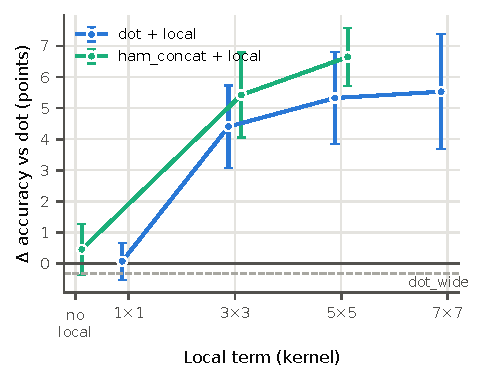
\includegraphics[width=\anchocolumna]{figuras/kernel.pdf}
  \caption{Accuracy difference against \var{dot} by size of the local term, with and without the \emph{pooling} branch of \var{ham\_concat} (seeds 0--4, 95~\% CI). The dashed line is the capacity control \var{dot\_wide}.}
  \label{fig:kernel}
\end{figure}

% Translated by scripts/tables_en.py from the Spanish table generated by scripts/ieee_tables.py a partir de los runs; no editar a mano.

\begin{table*}[!t]
\centering
\footnotesize
\caption{Ablation of the output terms on CIFAR-10 (seeds 0--4, 400 epochs). Paired differences against \texttt{dot} (80.04 $\pm$ 0.31) and against \texttt{dot\_local} ($3\times3$), with the number of favorable seeds in parentheses.}
\label{tab:ablacion}
\begin{adjustbox}{max width=\linewidth}
\begin{tabular}{lrcccrr}
\toprule
Variant & Params. & Accuracy (\%) & $\Delta$ vs \texttt{dot} & $\Delta$ vs \texttt{dot\_local} & Epoch $\geq$79 & s/epoch \\
\midrule
\texttt{dot\_local\_k1} & 119\,674 & 80.11 $\pm$ 0.31 & $+0.07$ [$-0.52$, $+0.67$] & $-4.33$ [$-5.43$, $-3.24$] (0/5) & 205 & 1.51 \\
\texttt{dot\_local} & 121\,210 & 84.44 $\pm$ 0.85 & $+4.40$ [$+3.08$, $+5.73$] & --- & 69 & 1.47 \\
\texttt{dot\_local\_k5} & 124\,282 & 85.36 $\pm$ 1.16 & $+5.32$ [$+3.84$, $+6.81$] & $+0.92$ [$-0.21$, $+2.05$] (5/5) & 53 & 1.49 \\
\texttt{dot\_local\_k7} & 128\,890 & 85.57 $\pm$ 1.27 & $+5.53$ [$+3.67$, $+7.38$] & $+1.12$ [$-0.24$, $+2.48$] (5/5) & 51 & 1.66 \\
\texttt{dot\_gate} & 128\,698 & 80.16 $\pm$ 0.50 & $+0.12$ [$-0.26$, $+0.51$] & $-4.28$ [$-5.57$, $-3.00$] (0/5) & 193 & 1.44 \\
\texttt{dot\_global} & 124\,298 & 80.17 $\pm$ 0.44 & $+0.13$ [$-0.33$, $+0.58$] & $-4.28$ [$-5.61$, $-2.94$] (0/5) & 199 & 2.14 \\
\texttt{dot\_local\_gate} & 130\,618 & 84.19 $\pm$ 0.22 & $+4.15$ [$+3.68$, $+4.62$] & $-0.26$ [$-1.52$, $+1.01$] (3/5) & 64 & 1.57 \\
\texttt{dot\_local\_global} & 126\,218 & 84.30 $\pm$ 0.21 & $+4.26$ [$+3.66$, $+4.85$] & $-0.15$ [$-1.12$, $+0.82$] (3/5) & 69 & 2.27 \\
\texttt{dot\_wide\_local\_k5} & 133\,982 & 85.65 $\pm$ 1.23 & $+5.61$ [$+4.26$, $+6.96$] & $+1.21$ [$-1.12$, $+3.54$] (4/5) & 61 & 1.52 \\
\texttt{ham\_concat\_local} & 130\,826 & 85.46 $\pm$ 1.32 & $+5.42$ [$+4.06$, $+6.79$] & $+1.02$ [$-1.24$, $+3.27$] (4/5) & 72 & 2.45 \\
\texttt{ham\_concat\_local\_k5} & 133\,898 & 86.68 $\pm$ 0.55 & $+6.64$ [$+5.71$, $+7.58$] & $+2.24$ [$+1.26$, $+3.22$] (5/5) & 50 & 2.46 \\
\bottomrule
\end{tabular}
\end{adjustbox}
\end{table*}


\section{Representative Attention Maps}
\label{sec:sup-mapas}
Fig.~\ref{fig:mapas} shows the CLS rollout of \var{dot} with two seeds, of \var{dot\_local\_k5} and of \var{ham\_concat\_local\_k5}, with the same color scale in each row. At a glance, the differences between variants are of the same order as the differences between two seeds of \var{dot}: in several images seed 1 of \var{dot} departs more from seed 0 than the models with a local term do. That is why the comparison is made quantitatively (Table~\ref{tab:mapas}). All divergences are small, because rollout accumulates the residual connection and produces smooth maps. Even so, the models with a local term have maps that are more reproducible across seeds than \var{dot} (JS of 0.0032--0.0055 versus 0.0062), and their distance to \var{dot} exceeds the between-seed variation of \var{dot} by a factor of 1.2 ($3\times3$) to 1.6 (\var{ham\_concat\_local\_k5}) and that of their own seeds by a factor of 1.8 to 3. In other words, the local term produces maps that differ from those of \var{dot} and are consistent across seeds. In an equivalent analysis of the fusions of the first family, by contrast, the distance of each variant to \var{dot} was of the same order as the variation between its own seeds: their maps were less reproducible, but not systematically different. The maps do not include the mixing done by the convolution (Section~\ref{sec:analisis}), so they only show how the attention part changes.

\begin{figure*}[!t]
  \centering
  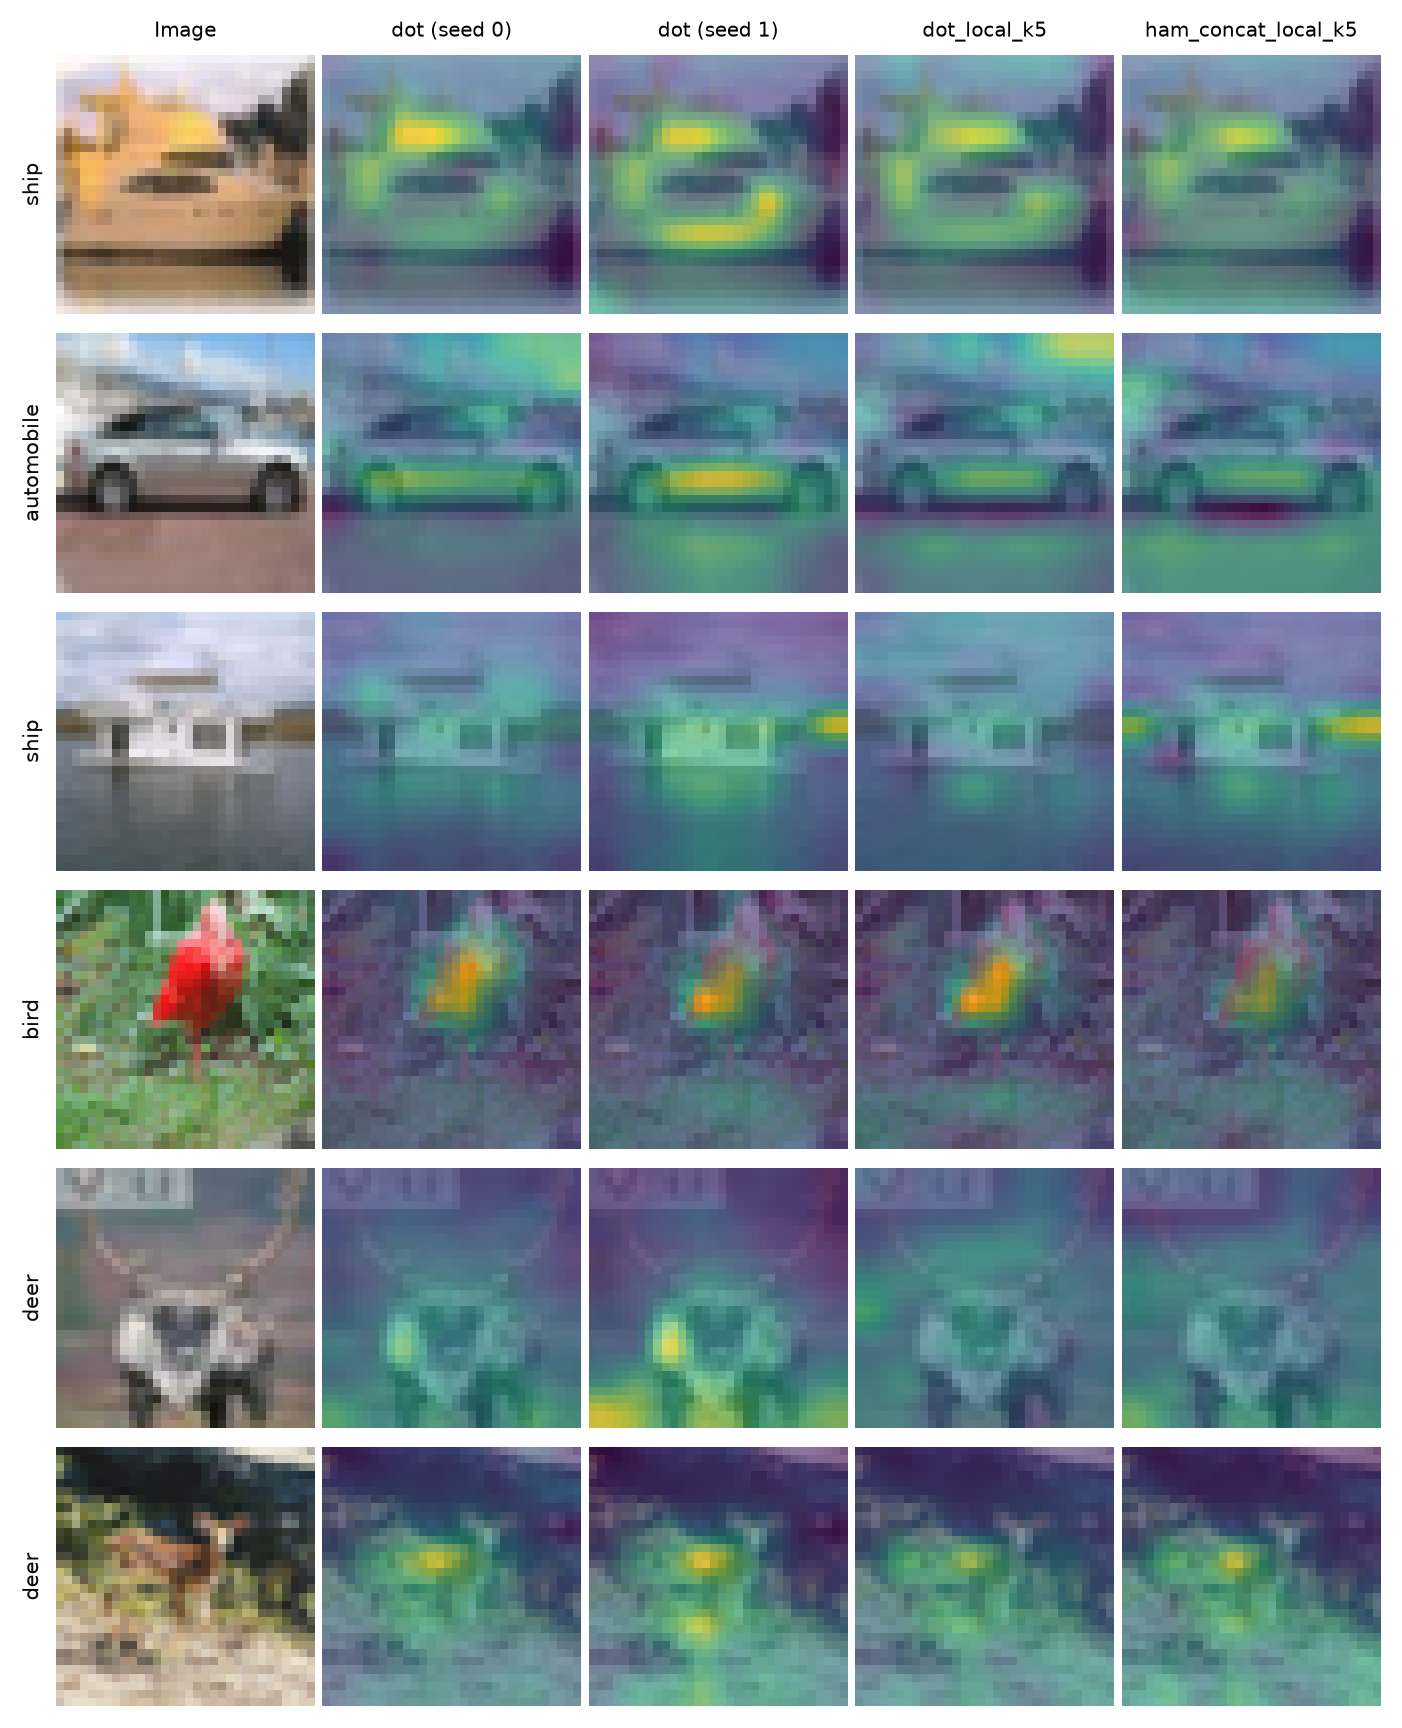
\includegraphics[width=0.62\textwidth]{figuras/mapas.png}
  \caption{CLS \emph{attention rollout} on six CIFAR-10 test images, with a common color scale in each row. The second seed of \var{dot} serves as a control: at a glance, the differences between variants are of the same order as those between two seeds of \var{dot}, so the maps alone do not distinguish the variants; Table~\ref{tab:mapas} compares them against the between-seed variation.}
  \label{fig:mapas}
\end{figure*}

% Translated by scripts/tables_en.py from the Spanish table generated by scripts/paper_tables.py a partir de los runs; no editar a mano.
\begin{table}[tbp]
\centering
\small
\caption{Jensen--Shannon divergence between CLS \emph{rollout} maps on CIFAR-10 (500 test images, seeds 0--4). Between seeds: mean over the 10 seed pairs of the variant. Against \texttt{dot}: same seed. Ratio: against \texttt{dot} divided by the between-seed variation of \texttt{dot}.}
\label{tab:mapas}
\begin{adjustbox}{max width=\columnwidth}
\begin{tabular}{lccc}
\toprule
Variant & JS between seeds & JS against \texttt{dot} & Ratio \\
\midrule
\texttt{dot} & 0.0062 & --- & --- \\
\texttt{dot\_local} & 0.0033 & 0.0076 & 1.22 \\
\texttt{dot\_local\_k5} & 0.0032 & 0.0096 & 1.54 \\
\texttt{ham\_concat\_local\_k5} & 0.0055 & 0.0100 & 1.60 \\
\bottomrule
\end{tabular}
\end{adjustbox}
\end{table}


\section{Sensitivity of the High-Mode Threshold}
\label{sec:sup-umbral}
The threshold of 85.5~\% that separates the two training modes (Section~\ref{sec:res-modos}) was chosen after observing the distribution. Table~\ref{tab:umbral} repeats the counts with thresholds between 85.0 and 86.0~\%. The direction of both comparisons is the same at every threshold: the $5\times5$ term enters the high mode more often than the $3\times3$ term, and the triad more often than its equal-capacity control. Their significance is not: $p$ ranges from 0.023 to 0.083 for $5\times5$ against $3\times3$, and from $<0.001$ to 0.152 for the triad against its control. The second comparison depends on the threshold because the triad also raises the low mode, to about 85~\%: with thresholds of 85.25~\% or lower, part of that mode is counted as high. The frequency comparisons are therefore exploratory, as stated in the main text.

% Translated by scripts/tables_en.py from the Spanish table generated by scripts/ieee_tables.py a partir de los runs; no editar a mano.

\begin{table*}[!t]
\centering
\footnotesize
\caption{Sensitivity of the high-mode frequency to the test-accuracy threshold on CIFAR-10. Seeds in the high mode / seeds; $p$: two-sided Fisher exact test. Left: 16 seeds (0--15); right: the triad and its equal-capacity control with 48 seeds (0--47).}
\label{tab:umbral}
\begin{adjustbox}{max width=\linewidth}
\begin{tabular}{lcccccccc}
\toprule
Threshold (\%) & \texttt{dot\_local} & \texttt{dot\_local\_k5} & \texttt{dot\_wide\_local\_k5} & Triad & $p$ ($5\times5$ vs.\ $3\times3$) & Triad & Control & $p$ \\
\midrule
85.00 & 3/16 & 9/16 & 8/16 & 14/16 & 0.066 & 44/48 & 24/48 & $<0.001$ \\
85.25 & 3/16 & 9/16 & 8/16 & 12/16 & 0.066 & 38/48 & 21/48 & $<0.001$ \\
85.50 (used) & 2/16 & 9/16 & 8/16 & 12/16 & 0.023 & 31/48 & 21/48 & 0.065 \\
85.75 & 2/16 & 9/16 & 8/16 & 11/16 & 0.023 & 29/48 & 21/48 & 0.152 \\
86.00 & 1/16 & 6/16 & 8/16 & 11/16 & 0.083 & 29/48 & 21/48 & 0.152 \\
\bottomrule
\end{tabular}
\end{adjustbox}
\end{table*}

